\documentclass[12pt, a4paper]{article}

\usepackage[utf8]{inputenc}
\usepackage[russian]{babel}
\parindent 0pt
\parskip 8pt
\usepackage{amsmath}
\usepackage{amssymb}
\usepackage{array}
\usepackage{floatrow}
\usepackage{float}
\usepackage[left=2.3cm, right=2.3cm, top=2.7cm, bottom=2.7cm, bindingoffset=0cm]{geometry} % headheight=0pt,
\usepackage{hyperref}
\usepackage{graphicx}
\usepackage{multicol}
\usepackage{fancyhdr} 
\usepackage{extramarks}
\usepackage[usenames,dvipsnames]{color}
\usepackage{titlesec}
\usepackage{tikz}
\definecolor{grey}{RGB}{128,128,128}

\pagestyle{fancy}
\fancyhf{}
\lhead{Билет № 1.1}
\chead{Элементарная база вычислительной системы: \\логические элементы, триггеры}
\rhead{\thepage}
\lfoot{made with Ы}
\cfoot{}
\rfoot{\today}
\renewcommand\headrulewidth{0.4pt}
\renewcommand\footrulewidth{0.4pt}

\titlespacing*{\section}{0pt}{5pt}{0pt}
\titlespacing*{\subsection}{0pt}{5pt}{0pt}
\titlespacing*{\subsubsection}{0pt}{5pt}{0pt}

\begin{document}

\section{Физические основы}

\subsection{Полупроводники*}
Многие вещества в кристаллическом состоянии не являются такими хорошими проводниками, как металлы, но их нельзя отнести и к диэлектрикам. Эти вещества - полупроводники. 

\subsubsection{Природа электрического тока в полупроводниках}
Экспериментально установлено, что электрический ток в полупроводниках не сопровождается переносом вещества - никаких химических изменений с ним не происходит. Отсюда следует, что носителями тока в полупроводниках, как и в металлах, являются электроны. Однако между полупроводниками и металлами имеются и глубокие различия.

Электроны металлов, находящиеся на внешних электронных оболочках (валентные электроны), сравнительно слабо связаны с атомами. Поэтому эти электроны (электроны проводимости) сравнительно легко отделются от атомов и образуют электронный газ, концентрация которого очень велика. Эти электроны принадлежат всей кристаллической решетке и легко перемещаются по всему проводнику. Именно с этим связана высокая проводимость металлов.

В полупроводниках валентные электроны значительно сильнее связаны с атомами. Поэтому концентрация электронов проводимости при комнатной температуре в полупроводниках незначительна.

\subsubsection{Донорные и акцепторные примеси}
Свойства полупроводников сильно зависят от содержания примесей.

Пусть, например, в кристалле кремния имеется примесь пятивалентных электронов мышьяка, которые замещают в узлах кристаллической решетки атомы кремния. Пятивалентный атом мышьяка вступает в ковалентные связи с четыремя атомами кремния (у кремния валентность четыре), а его пяый электрон оказывается незанятым в связях.

Энергия, необходимая для отрыва пятого электрона от атома мышьяка в кристалле кремния значительно больше энергии, необходимой для отрыва электрона от атома кремния. Поэтому при комнатной температуре значительная часть атомов мышьяка лишается одного из своих электронов и становится положительными ионами.

Положительный ион мышьяка не может захватить электрон у одного из соседних атомов кремния, т.к там энергия связи больше. Поэтому дырочной проводимости нет. Примеси, поставляющие электроны проводимости без возникновения равного им количества "дырок" называются \textit{донорными}.

Полупроводниковый кристалл, содержащий донорные примеси, называется \textit{электронным} полупроводником или полупроводником $n$-типа.

Логично, что если добавим в кристалл примесь трехвалентного элемента, то получим избыток "дырок". Такие примеси называются \textit{акцепторными}, а полупроводниковые кристаллы, содержащие такие примеси, называются \textit{дырочными} полупроводниками или полупроводниками $p$-типа.

\subsection{p-n-переход*}
Электронно-дырочный переход, или, сокращенно $p-n$-переход, является границей, разделяющей области с дырочной($p$) и электронной($n$) проводимостями в одном и том же монокристалле.

Пограничная область раздела полупроводников с различным типом проводимости (она называется \textit{запирающим слоем}) в связи с уходом свободных электроном практически превращается в диэлектрик.

Если $p-n$-переход соединить с источником тока так, чтобы с его положительным полюсом была соединена область с электронной проводимостью, то электроны в $n$-проводнике и "дырки" в $p$-проводнике удаляются внешним полем от запирающего слоя в разные стороны, увеличивая его толщину. Сопротивление $p-n$-перехода велико, сила тока мала и почти не зависит от напряжения.

Если $p-n$-переход соединить с источником тока так, чтобы с его положительным полюсом была соединена область с "дырочной" проводимостью, то переходы основных носителей тока через $p-n$-переход облегчаются. Двигаясь навстречу друг-другу, носители входят в запирающий слой, уменьшая его сопротивление.

Такие дела.

\subsection{Транзисторы}
Транзистор - полупроводниковый прибор с двумя $p-n$-переходами и тремя выводами.
\subsubsection{Биполярный транзистор*}
С помощью соответствующих примесей в кристалле германия или кремния создают три области: между двумя областями $p$-типа создают слой 2 с проводимостью $n$-типа, называемый \textit{базой} (рис. 8.37). Одна из разделенных областей называется \textit{эмиттером}, а вторая \textit{коллектором}. Таким образом, между эмиттером и базой, а также коллектором и базой создаются два $p-n$-перехода 4 и 6, пропускные направления которых противоположны. На рисунке 8.38 показано условное обозначение биполярных транзисторов.\\
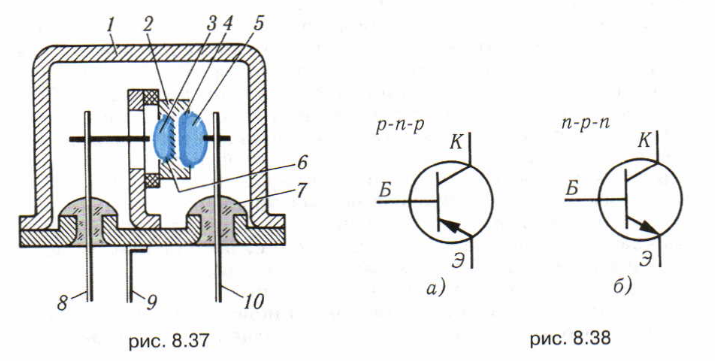
\includegraphics[scale=0.5]{./images/polTransistor.png}
\subsubsection{Полевые транзисторы}
Существуют два вида полевых МОП-транзисторов: n-МОП и p-МОП
(по английски n-MOS и p-MOS, что произносится как н-мосс и пи-мосс).
На Рис. 1.29 схематически показано сечение каждого из этих двух
типов транзисторов так, как будто мы распилили кристалл и теперь смотрим на транзистор сбоку. В транзисторах n-типа, называемых
n-МОП, области, где расположены полупроводниковые примеси
n-типа – в свою очередь называемые истоком (source) и стоком
(drain) – находятся рядом с затвором (gate), причем вся эта структура
размещается на подложке p-типа. В транзисторах же p-МОП и исток,
и сток – это области p-типа, размещенные на подложке n-типа.
Полевой МОП-транзистор ведет себя как переключатель, управляемый
приложенным к нему напряжением. В таком транзисторе напряжение
перехода создает электрическое поле, включающее или выключающее
линию связи между источником и стоком. Термин полевой транзистор
(field effect transistor) является прямым отражением принципа работы
такого устройства. Знакомство с работой полупроводниковых устройств
мы начнем с изучения n-МОП-транзистора.\\
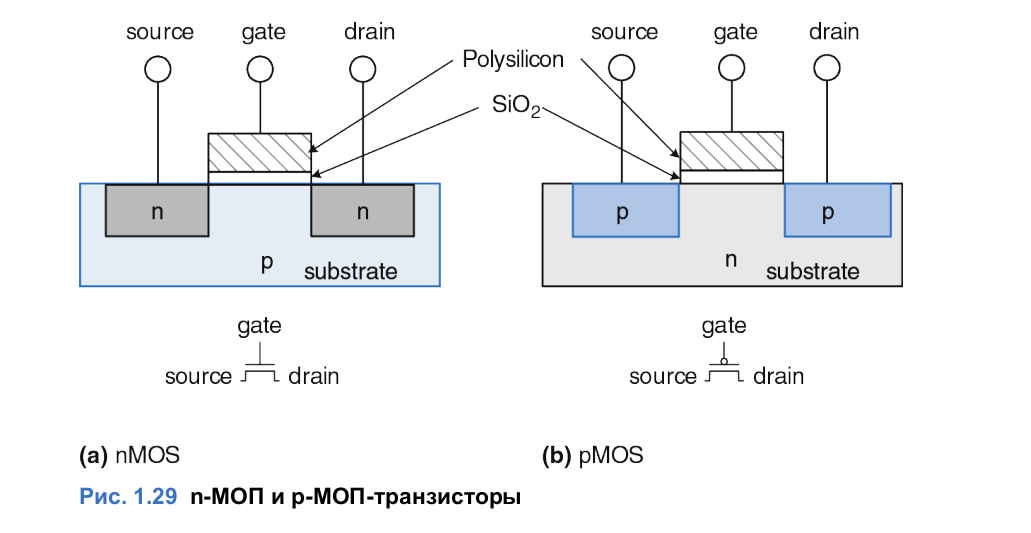
\includegraphics[scale=0.5]{./images/1_29.png}\\
Подложка n-МОП транзистора обычно находится под напряжением
земли GND, которое является минимальным напряжением в системе.
Для начала рассмотрим случай, когда, как показано на Рис. 1.30 (a),
напряжение на затворе также равно 0 В. Диоды между истоком или
стоком и подложкой находятся в состоянии, называемым обратным
смещением (reverse bias), поскольку напряжение на истоке и стоке не
является отрицательным. В результате этого канал для движения тока между истоком и стоком остается закрытым, а транзистор выключенным. Теперь рассмотрим ситуацию, когда напряжение на затворе повышается до V DD – так, как показано на Рис. 1.30 (b).Если приложить положительное напряжение к затвору (верхней пластине конденсатора), то это создаст электрическое поле между затвором и
подложкой, в результате в зоне между истоком и стоком под слоем
оксисла формируется избыток электронов. При достаточно высоком
напряжении на нижней границе затвора накапливается настолько много
электронов, что область с полупроводником p-типа превращается в
область с полупроводником n-типа. Такая инвертированная область
называется каналом (channel). В этот момент в транзисторе образуется
область проводимости от источника n-типа, через каналы n-типа к стоку
n-типа, и через этот канал электроны могут беспрепятственно
перемещаться от истока к стоку. Транзистор включен.\\
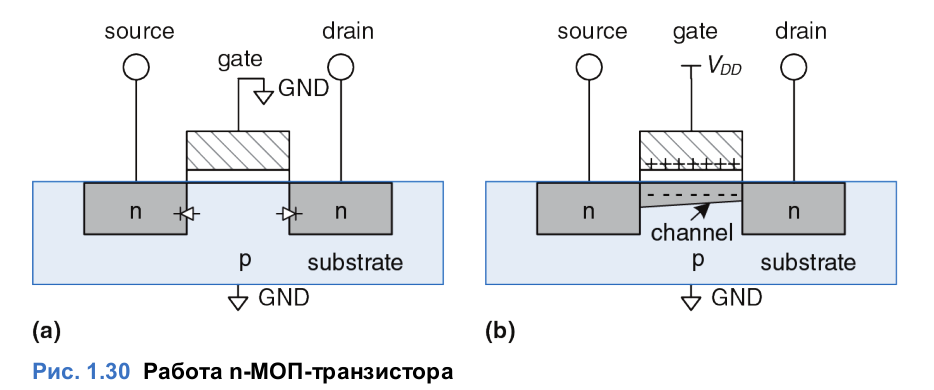
\includegraphics[scale=0.5]{./images/1_30.png}
\section{Логические элементы}
\subsection{Логические вентили}
\textbf{Логический вентиль} - базовый элемент цифровой схемы, преобразующий входные сигналы в выходные в соответствии с какой-либо булевой функцией. В устройствах реализуется с помощью транзисторов.\\
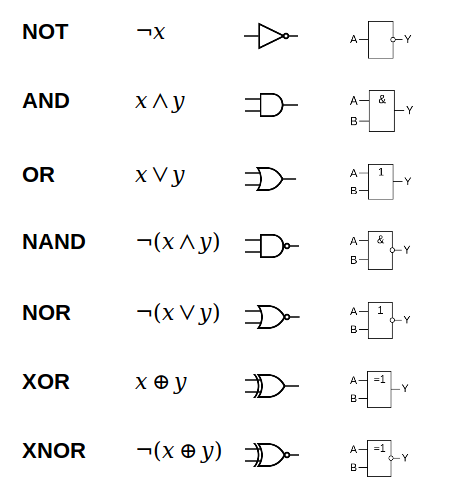
\includegraphics[scale=0.4]{./images/logicGates.png}

\subsection{Реализация базовых элементов с помощью транзисторов}
\begin{figure}[h]
  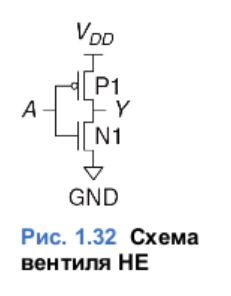
\includegraphics[width=0.3\linewidth]{./images/NOT.png}
  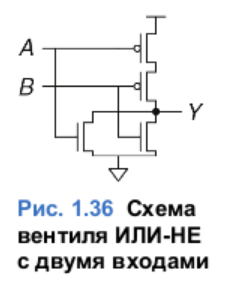
\includegraphics[width=0.3\linewidth]{./images/NOR.png}
  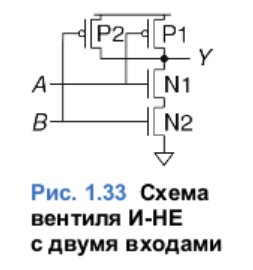
\includegraphics[width=0.3\linewidth]{./images/NAND.png}
  \label{fig:tr-el}
\end{figure}

\section{Комбинаторные схемы}
\textbf{Комбинаторные схемы} - схемы, зависящие только от своих входов.
\subsection{Мультиплексор}
\textbf{Мультиплексор} - схема с $2^n$ входами, одним выходом и $n$ линиями управления, которые позволяют выбрать один из входов. Выбранный вход соединяется с выходом. На рисунке показана схема восьмивходового мультиплексора.\\
\begin{figure}[h!]
    \centering
    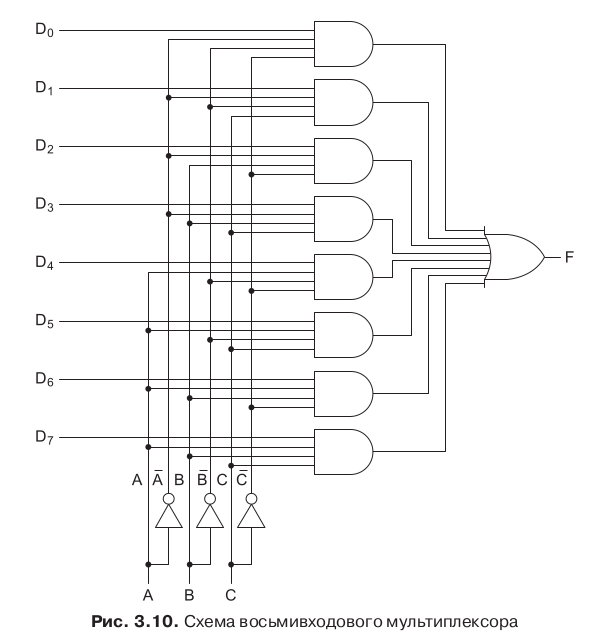
\includegraphics[width=0.4\linewidth]{./images/3_10.png}
    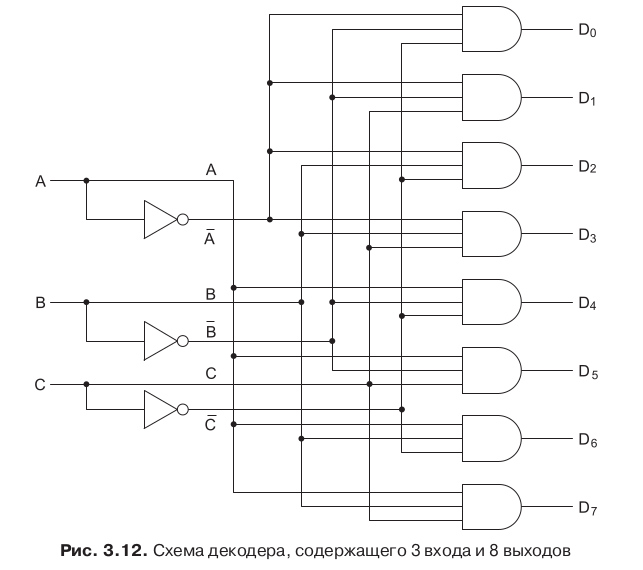
\includegraphics[width=0.4\linewidth]{./images/3_12.png}
\end{figure}
\subsection{Демультеплексор}
\textbf{Демультиплексор} соединяет единственный входной сигнал с одним из $2^n$ выходов в зависимости от значений сигналов в $n$ линиях управления. Если бинарное значение линий управления равно $k$, то выбирается выход $k$.
\subsection{Дешифратор (декодер)}
\textbf{Дешифратор} - схема, которая получает на входе $n$-разрядное число и использует его для того, чтобы выбрать (т.е. установить в значение 1) один из $2^n$ выходов.
\section{Арифмитические схемы}
\subsection{Полусумматор}
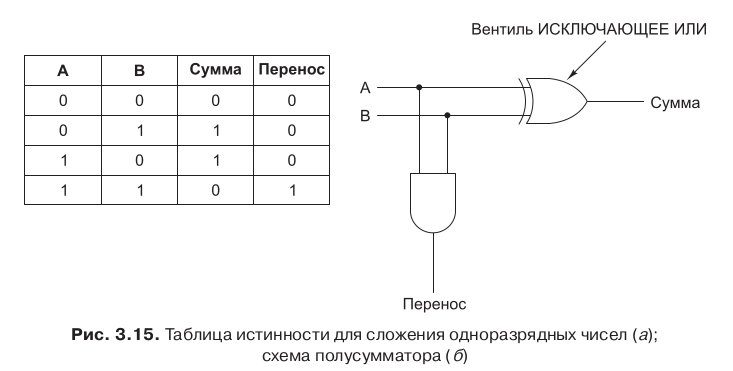
\includegraphics[scale=0.6]{./images/3_15.png}
\subsection{Сумматор}
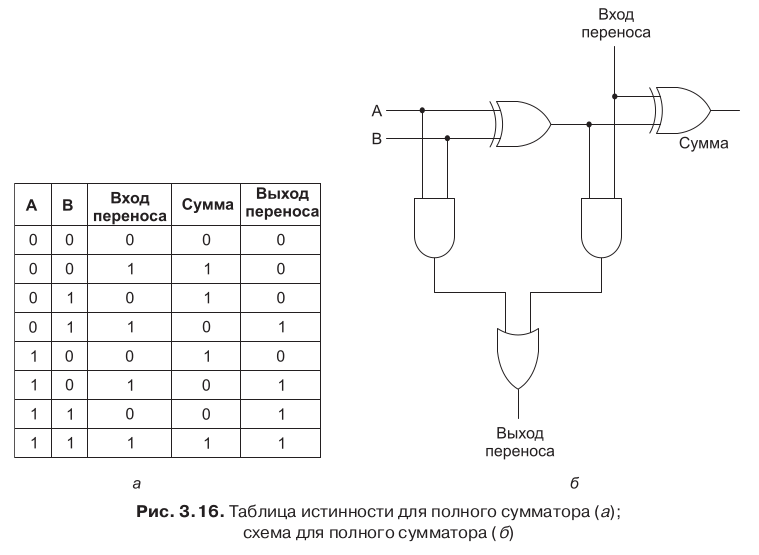
\includegraphics[scale=0.6]{./images/3_16.png}
\section{Последовательные схемы}
\textbf{Последовательная схема} зависит не только от своих текущих входов, но и от своего текущего состояния.
\subsection{Триггеры}
Вообще существуют триггеры (срабатывают по фронту или спаду импульса синхронизации) и защелки (срабатывают по уровню импульса синхронизации), но Скаков в разницу между ними не умеет (а вот Таненбаум умеет). Поэтому в этом конспекте все штуковины называются триггерами, даже когда они на самом деле защелки :(
\subsubsection{RS-триггер}
Схема, изображенная на рис. 3.20, а, называется \textbf{RS-триггером}. У нее есть два входа: S (Setting — установка) и R (Resetting — сброс).\\
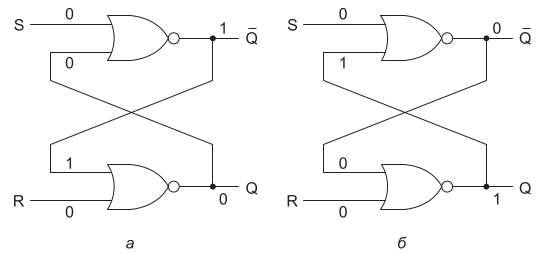
\includegraphics[scale=0.4]{./images/3_20.png}%
\begin{tabular}{ |c|c|c| } 
 \hline
 R & S & Q \\ 
 \hline
 0 & 0 & Q \\ 
 \hline
 0 & 1 & 1\\ 
 \hline
 1 & 0 & 0 \\
 \hline
 1 & 1 & Forbidden \\
 \hline
\end{tabular}
\subsubsection{Синхронный RS-триггер}
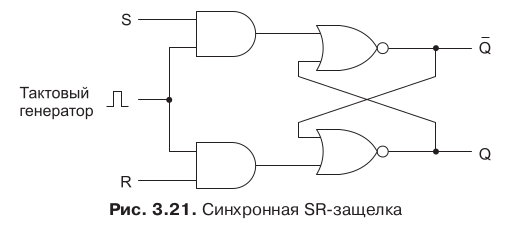
\includegraphics[scale=0.6]{./images/3_21.png}\\
Эта схема имеет дополнительный синхронизирующий вход, который по боль-
шей части равен 0. Если этот вход равен 0, то оба выхода вентилей И равны 0,
и независимо от значений S и R триггер не меняет свое состояние. Когда зна-
чение синхронизирующего входа равно 1, действие вентилей И прекращается,
и состояние триггера становится зависимым от S и R.
\subsubsection{Синхронный D-триггер}
Чтобы разрешить ситуацию с неопределенностью SR-триггера (неопределенность
возникает в случае, если S = R = 1), нужно предотвратить ее возникновение.\\
Пусть теперь у RS-триггера будет один вход, D.\\
D = 0 -> R = 1, S = 0\\
D = 1 -> R = 0, S = 1\\
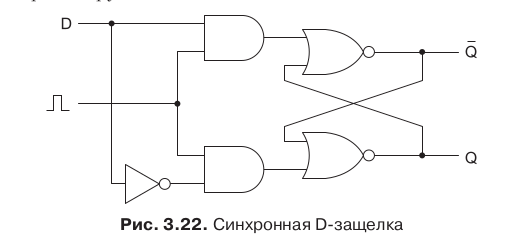
\includegraphics[scale=0.6]{./images/3_22.png}
\subsubsection{JK-триггер}
\begin{figure}[h!]
    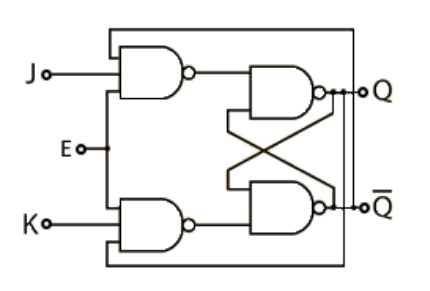
\includegraphics[width=0.5\linewidth]{./images/3_24.png}
    \caption{JK-триггер. Имеет одну большую проблему: если сигнал синхронизации подавать достаточно долго, то значение на выходах изменится до того, как сигнал спадёт. И выходы инвертируются ещё раз.}
    \label{fig:my_label}
\end{figure}
\begin{figure}[h!]
    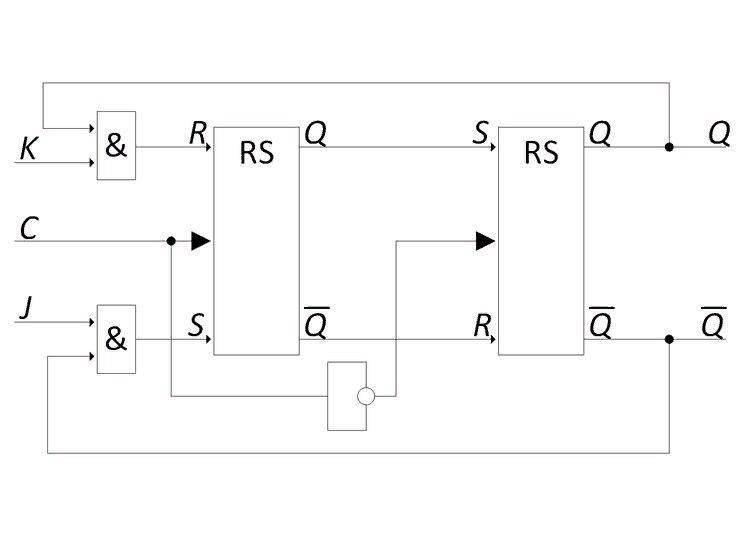
\includegraphics[width=0.4\linewidth]{./images/JK.jpg}
    \caption{JK-триггер Скакова (можно прогуглить что-то похожее как Master-Slave JK Flip Flop). Срабатывает только по спаду импульса синхронизации, если сигнал удерживать - значение не изменится}
    \label{fig:my_label}
\end{figure}
При J = 0, K = 0 -> сохраняет значение\\
При J = 0, K = 1 -> дает на выходе 0\\
При J = 1, K = 0 -> дает на выходе 1\\
При J = 1, K = 1 -> инвертирует значение\\
\begin{table}[h!]
    \centering
    \begin{tabular}{c|c|c|c|c|c|}
         & J & K & C & $Q_1$ & $Q$ \\
         & 0 & 1 & 1 & 0 & 0\\
         & 0 & 1 & 0 & 0 & 0\\
         & 1 & 1 & 0 & 1 & 0\\
         & 1 & 1 & 1 & 1 & 1\\
         & 1 & 1 & 0 & 0 & 1\\
         & 0 & 0 & 0 & 0 & 1\\
         & 0 & 0 & 1 & 0 & 0
    \end{tabular}
    \caption{\textbf{Как сломать JK-триггер с перемещенным инвертором?}\\$Q_1$ - выход первого RS-триггера}
    \label{tab:my_label}
\end{table}
\subsubsection{T-триггер}
При T = 0 не изменяет значения, при Т = 1 меняет значение на противоположное.\\
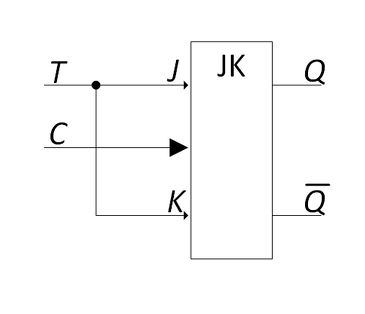
\includegraphics[scale=0.6]{./images/T.jpg}\\
\section{Регистры}
Существуют различные конфигурации триггеров. На рис. 3.26 показано, как во-
семь триггеров объединяются для формирования 8-разрядного регистра. Регистр
получает 8-разрядное входное значение (I0 – I7) при изменении синхронизирующего сигнала CK. Все синхронизирующие линии связаны с одним входным
сигналом CK, чтобы при изменении состояния CK регистр получал новое 8-разрядное значение данных с входной шины. Триггеры запускаются при переходе от 0 к 1. Все восемь сигналов очистки тоже объединены, поэтому когда сигнал сброса CLR переходит в состояние 0, все триггеры переходят в состояние 0. Если вам не понятно, почему синхронизирующий сигнал CK инвертируется на входе, а затем инвертируется снова в каждом триггере, то ответ прост: входной сигнал не имеет достаточной мощности, чтобы запустить все восемь триггеров; входной инвертор на самом деле используется в качестве усилителя.\\
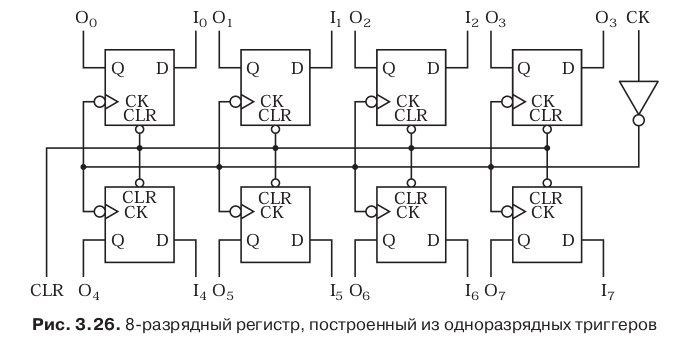
\includegraphics[scale=0.6]{./images/3_26.png}
\section{Счетчик}
\textbf{Счетчик} - устройство, предназначенное для счета количества тактов, используется, например, для деления частоты и в схемах таймеров, а также для выбора инструкций из ПЗУ в микропроцессорах.\\
Простой двоичный счетчик реализуется на основе T-триггеров.\\
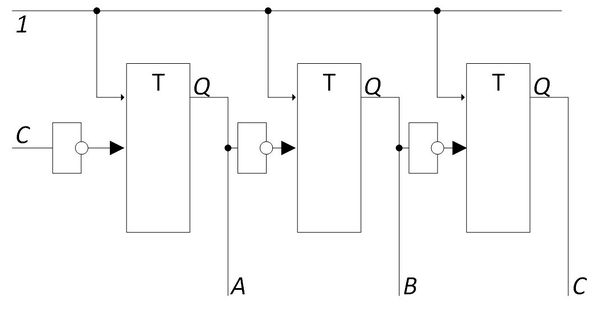
\includegraphics[scale=0.4]{./images/counter.jpg}\\
Если долго смотреть на картинку, можно даже понять как именно эта штука работает.
\section{Источники информации}
\begin{enumerate}
    \item Разделы про полупроводники и биполярные транзисторы - учебник физики 10 класс А.А. Пинский, О. Ф. Кабардин
    \item Полевые транзисторы, базовые элементы с помощью транзисторов - Д. Харрис, С. Харрис "Цифровая схемотехника и архитектура компьютера"
    \item Комбинаторные, арифметические и последовательные схемы - Э. Таненбаум "Архитектура компьютера"
    \item Последовательные схемы, регистры, счетчик - конспекты прошлого года + википедия
\end{enumerate}
\end{document}